\documentclass[12pt,a4paper,openright,twoside]{book}
\usepackage[utf8]{inputenc}
\usepackage{disi-thesis}
\usepackage{code-lstlistings}
\usepackage{notes}
\usepackage{shortcuts}
\usepackage{acronym}
\usepackage{float}

\school{\unibo}
\programme{Corso di Laurea Magistrale in Ingegneria e Scienze Informatiche}
\title{Overview, study, and comparison of open source automation tools:\newline Ansible, Salt, Chef, Puppet}
\author{Alberto Donati}
\date{\today}
\subject{Distributed Systems}
\supervisor{Prof. Giovanni Ciatto}
%\cosupervisor{Dott. CoSupervisor 1}
%\morecosupervisor{Dott. CoSupervisor 2}
\session{Unica}
\academicyear{2022-2023}

% Definition of acronyms
%\acrodef{IoT}{Internet of Thing}
%\acrodef{vm}[VM]{Virtual Machine}


\mainlinespacing{1.241} % line spacing in mainmatter, comment to default (1)

\begin{document}

\frontmatter\frontispiece

\begin{abstract}
    Considering that companies have an increasing number of servers connected to the network, IT professionals increasingly find themselves with machines on which to perform the same tasks.
    Therefore, systems that could automate tasks on large numbers of machines in parallel have been created and are increasingly being used.
    This thesis aims to compare and evaluate different server automation tools, analyzing their features, advantages, and disadvantages.
    It will then go on to provide a summary overview of the reasons why professionals choose one alternative over another.
\end{abstract}

%\begin{dedication} % this is optional
%Optional. Max a few lines.
%\end{dedication}

%\begin{acknowledgements} % this is optional
%Optional. Max 1 page.
%\end{acknowledgements}

%----------------------------------------------------------------------------------------
\tableofcontents   
\listoffigures     % (optional) comment if empty
\lstlistoflistings % (optional) comment if empty
%----------------------------------------------------------------------------------------

\mainmatter

%----------------------------------------------------------------------------------------
\chapter{Introduction}
\label{chap:introduction}
%----------------------------------------------------------------------------------------

Considering the last decades, the number of servers increased, computing capacity is increasing more and more and technologies are growing.


So, now IT companies need also technologies to manage the infrastructure they have, which could simplify and organize the jobs on servers.


There are a lot of repetitive tasks when it is needed to install and configure a server, so there are now tools to simplify it a lot and also make an automation on it.

These technologies are usually called "automation tools".

Considering different DevOps technologies, this document aims to study and compare some open source technologies about automation.

That document will be useful for IT students, teachers and enthusiasts who wish to manage their IT environment differently.

It will be a starting point to see what is an automation tool, different types of ways to automate with these technologies, see some examples and also see overviews and comparisons.

\section{Metology}
Starting from some technologies that it is already known, it will search for technologies similar to them.


Also, sites and theses that talk about automation will be beginning to see what technologies exist.


There will be a focus on "popular" tools in these years. Searching for technologies just created will not be the scope, and also finding technologies too old might result in not being useful for real use.


Technologies based on open source projects with a free version and a community-oriented license will be considered.


There are some technologies properties of Amazon, Google and Microsoft, even if they might be described, they will not be the focus of the document.


That study also searches for technologies that could be useful for multipurpose scope, always related to automation.


These tools must have a solid user base. Also, It does not search for a particular language or a single way to manage machines (for example agent-agentless).


There are no limitations about the languages used in the tools for automation or abot the language for the tool project itself. Some base automations on YAML language (Salt, Ansible), and others on Ruby and/or relative DSL (Chef, Puppet).

\section{Explanation of the structure}
Initially, there will be a brief description of what the automation tools are and who uses them.


Also, there will be a brief explanation about Open Source, and its importance for the projects in our use case.


For each technology, there will be a little historical view, a little study about the open source project, the trend of the language, the community and the support.


There will be a description of the tool and its components.


Also, some info on installation and examples.


Considering that automation could be easily integrated with CI/CD, it will be searching for some sort of automatic test and checks of the technology.


Considering this research and other sources, there will be a little description of the pros and cons.


At the end, there will be a summary of the research done writing that document, and tables or similar mixing different technologies.

The structure will be something like this:

\begin{itemize}
    \item Introduction
    \item State of the art (what are automation tools, who uses, open source)
    \item for each automation tool:
    \begin{itemize}
    \item History of the technology
    \item Purpose of the technology
    \item Community, maintenance and support
    \item Main technology components
    \item Installation and examples
    \item How to test the technology
    \item Pros and Cons
    \end{itemize}
    \item Conclusions (Considerations and comparisons)
\end{itemize}


\chapter{State of the art}

\section{What are automation tools}
We could consider in some way that for DevOps purposes all the job we need to execute is expressed in the form of code\cite{learnDevOps}.


And also the configuration of servers and installations of software could do that.


Automation tools are software tools that allow you to manage, monitor, and automate operations on a large number of servers. These systems can include features such as automatic provisioning, configuration management, service orchestration, performance monitoring, and troubleshooting.


An example of these systems is \textbf{Ansible}, which uses an agentless management model to connect to servers and perform automation tasks. Other examples include Puppet, Chef, and SaltStack, which offer similar features but use different approaches for server management.


These automation systems can be particularly useful in environments with a large number of servers, where manual management of each server would be inefficient and prone to errors. Through automation, organizations can improve operational efficiency, reduce errors, and free up IT staff to focus on different works.


Automation systems aim to simplify the execution of repetitive tasks.

\section{Who uses automation tools}
Automation tools could be useful for a single user who wishes to simplify some tasks in the home running server (or cloud), to IT companies or Universities from a few to thousands of servers.

Some automation tools are simpler than others, for example starting from the structure of the language used to create automations.

Some could be used by beginners in IT and others require OOP knowledge of languages like Ruby.

\section{When it makes sense (or doesn't make sense) to automate operations}
Some questions help to understand when an automation tool could be a great choice:
\begin{itemize}
    \item Does It need to do that job more than once?
    \item How much time did I spend to create that automation?
    \item Create that automation will save me time or is time-consuming and not useful?
    \item What is the probability that I need to do that job another time in the future?
    \item How much is the ability to use that tool?
\end{itemize}

For example, in the case that building a very particular Linux machine with a list of packages, even if only one is needed, it could be useful because If in the future another installation of the same configuration is needed, it is possible to reinstall all the system in a few steps.


At the same, if I need to install a few packages on hundreds of servers, it will be a saving time procedure.


On the other hand, we might consider also the time spent on learning the technology, if I already know that, I could automate also very simple jobs because it is used to automate all.


If it is a beginner, there are some stuff that probability has no sense to automate because the effort and time are not worth it.


When someone knows a tool enough, it is possible to also expand the automation for more complex jobs.

\section{What are the main tools}
Some of the tools used by the community for automation, which try to reply to the scope indicated above are:

\begin{itemize}
    \item Ansible
    \item Salt
    \item Chef
    \item Puppet
\end{itemize}

Every technology has some differences considering for example language to write automation, learning curve, necessity of demons, connection with machines and so on.

\section{OpenSource and Closed Source, when OpenSource becomes Closed for some use cases}
Nowadays there are a lot of companies that acquires strategically some important business related to Open Source projects.


In the last years, for example, Ansible was acquired by RedHat in 2015, GitHub was acquired by Microsoft in 2018, Salt was acquired from VMware in 2020.


Even if there are some problems when a company acquires a company related to a big open-source project, it doesn't mean that the technology is worse because there are companies that make a profit from it.

Usually, big tech companies that acquire others related to open source contribute to spreading and improving the technology.


It is possible to consider one of the most important examples of that in Ubuntu.


Ubuntu is one of the most popular Linux distributions, Ubuntu has great community support and behind it is the company Canonical.


Canonical helps and contributes to Ubuntu distribution but also sells some products related like support, differences updates, and infrastructures.

An example of an automation tool could be Red Hat which offers Ansible Automation Platform.
Red Hat describes it as an end-to-end automation platform able to scale across the entire enterprise that is useful to configure systems, deploy software, and orchestrate advanced workflows.\cite{ansibleAutomationPlatform}
Automation controller is a part of Ansible Automation Platform, and there is a sort of community-supported alternative called "AWX"\cite{ansibleAwxAAP}.
Red Hat explains that Automation controller "is produced by taking selected releases of AWX, hardening them for long-term supportability, and making them available to customers as a hosted service within Red Hat Ansible Automation Platform"\cite{ansibleFaq}.

Also Salt has open source versions and an enterprise version. The open source is free and usable via a command-line interface.
The paid enterprise edition (but the prices are not available to the public), SaltStack Enterprise, adds some features such as GUI and support for Windows and MacOS.
Salt offers professional services to help customers integrate with third-party systems, also, the Salt Enterprise API has many more features than the free version.\cite{saltTechTarget}


So, when a company makes a big contribution to an open-source project there could be some negative implications ( for example regarding support or licenses), but the community nonetheless takes benefits.

\chapter{Ansible}

\section{The beginning of Ansible}

Michael DeHaan define Ansible:
"Ansible is a configuration management tool, deployment tool, and ad-hoc task execution tool all in one."


The observation that formed the basis of Michael DeHaan's idea was that several online stores used separate tools for configuration, deployment, and yet another for task execution. This was because there was not one technology that could perform all these functions.


He also wanted Ansible to be as extensible as possible, that is, modules could be written in any language that could return JSON or key-value pairs.

One of the basic concepts that Micheal specified from the beginning was that configuration should be extremely simple, so without using configuration files, daemons and databases. Ansible from the beginning used a file with the machines that were to be managed written on it. Only the machines described in that file were managed, in case they were not included they would not be managed.

Quoting Micheal on his motivations for creating Ansible:


"While part of starting Ansible was to show the world there was an easier way -- to take those lessons from Red Hat, the field, and a long history of building systems management applications -- it was mostly to build the tool that (A) I actually wanted to use, and (B) was a tool that you could not use for six months, come back to, and still remember. I couldn't bring myself to be settled with the tools we had to use, it was too frustrating. As a developer myself, I wanted to write development code, I didn't want to spend 50\% of my time fighting with the automation tooling and have the automation itself be a source of frustration. I wanted to help all of these IT environments I was finding myself in, and also help myself as a consumer of those environments."

The motivation of Micheal about the project was:


"As a software developer, I myself can emphasize -- the software design/development/testing process is frequently painful, and I would rather think of infrastructure as being data-driven. Data is supposed to be simple, programs are often not. This is why I made Ansible."

\subsection{History}
In 2006 Michael DeHaan was working at Red Hat's Emerging Technologies group, a research unit under Red Hat. Emerging Tech was created specifically as a place where people could work on virtually anything they thought people needed.


Still those years, RedHat was very interested in configuration management. An early prototype of application virtualization management used Cobbler for provisioning the base operating system and Puppet for configuring virtual machines.


This project did not take off and Michael DeHaan attributed the cause to the fact that it was complex to write the details under virtual applications, but Red Hat virtualization was also still in its early days.


Greg DeKoenigsberg was a Fedora community character and created a group with Michael DeHaan, Adrian Likins and Seth Vidal (author of yum). They wanted to create another very democratic open-source project in Red Hat, one that could have a wide variety of contributors and solve new problems. They thought back to busrpc. This project existed because it filled the gaps between Cobbler and Puppet. Cobbler could provide a system, and Puppet could put in configuration files, but because Puppet was too declarative you couldn't use it to do things like restart servers or do all the "ad hoc" tasks. In the past, Red Hat was exploring CIM, but there were not many good implementations of API support for Linux, so it would not be possible to build an open source project that would be able to have community success around CIM. The idea that was followed was to create an API-like channel for managing applications to configure systems, This idea was called Func.


Func was based on a central server reaching out to a remote node to send automation orders. It was called the central server "overlord" and each of the remote machines "minions." 


Other clones of Func were also created. Fabric and Capistrano also existed, but the team of Func wanted something more of an API and less of a script. Func was later used by Tumblr, and Steve Salesvan, who was interning at Red Hat at the time, continued to maintain it for Tumblr.


Michael therefore wanted to build a configuration management system on top of Func, tentatively called "Remote Rocket Surgery."


Cobbler, Puppet and Func formed some of the earliest DevOps-friendly automation tools, with Cobbler sometimes doing the provisioning and Func being used to launch Puppet.


After leaving RedHat and a brief term at Puppet, Micheal saw that the language often divided potential users and that the most important thing in automation tools, simplicity, should be a priority.


So Ansible began as a project at the beginning of 2012. It took off quickly due to many sysadmins and developers knowing Micheal.
Also, people from Fedora Infrastructure, replaced their Puppet automation with Ansible so Fedora helped Ansible to grow and also used it as a test platform.


Like Func, it pursues a "batteries included" philosophy, allowing everyone to contribute to the main modules and forming an active community of users.


After a period when Micheal was working on the automation of OpenStack with Puppet, the project started to take off on GitHub, and soon the company was founded.


Ansible increased and Micheal and others had a good-sized company supporting it and more importantly, building great products on top of it.


In 2015 Ansible was acquired from RedHat\cite{ansibleRedHat}.


Now, Ansible is currently one of the most used automation tools.

\section{Purpose of the technology}
Ansible is a technology used for automation. It allows any environment to manage the automation of commands on other machines.


The files used for the description and therefore the execution of the scripts are called Playbooks.


Ansible is based on the Python language, so it is cross-platform.


Usually, its use is recommended in a Linux environment, but some features are slightly different in a Windows environment.


Considering that most servers have a Linux kernel, the tests will focus on a Linux environment.


Ansible is ideal for managing IT environments, as it can automate tasks on a multitude of nodes simultaneously.

\subsection{Best points of Ansible}
\begin{itemize}
    \item \textbf{Simple}: As syntax, the files are described in YAML language. YAML is easy to understand by those who have minimal knowledge of programming languages and is often used for configurations. In addition, most configuration management software is characterized by an agent and a server from which to start the orchestration. In this case, Ansible's agentless management makes it easy to manage machines.
    \item \textbf{Fast}: Ansible, in addition to having a low learning curve, has a fast configuration, not having agents that must be constantly active on the host machines. Ansible connects directly to the host machines via SSH, and it is enough to have Python installed on the host machines.
    \item \textbf{Efficient}: Considering that Ansible does not have active agents, this does not consume extra resources in the hosts where the automatisms are executed. Ansible takes space and resources only during the execution of the activity on the controlled node.
    \item \textbf{Secure}: Considering that the connection from the manager to the controlled node is via SSH, no extra open ports are required.
\end{itemize}

\section{How the tool is shown to the community}

\subsection{Who supports and maintains the project}

\subsection{Statistics}
Ansible has 
\begin{itemize}
    \item 60.1k stars
    \item 1.9k watcher
    \item 24k fork
    \item 500 issue with $>$30k closed
    \item $>$300 pull request
    \item $>$5000 contributors
    \item 31.8k projects use it as a dependency
\end{itemize}

We could consider the community very active, considering also that every few days a new issue appears.

\subsection{Community way to help and improve}
If someone with to be involved in the project there is the official page that explains\cite {ansibleGithub}.

\begin{itemize}
    \item Read Community Information for all kinds of ways to contribute to and interact with the project, including mailing list information and how to submit bug reports and code to Ansible.
    \item Join a Working Group, an organized community devoted to a specific technology domain or platform.
    \item Submit a proposed code update through a pull request to the devel branch.
    \item Talk to us before making larger changes to avoid duplicate efforts. This not only helps everyone know what is going on, but it also helps save time and effort if we decide some changes are needed.
    \item For a list of email lists, IRC channels and Working Groups, see the Communication page
\end{itemize}

There is also a sort of community-based platform to share collections and roles, called Ansible Galaxy\cite{ansibleGalaxy}.
The documentation of Ansible also includes instructions to use Galaxy for the projects.
An Ansible-related open source project is AWX which "provides a web-based user interface, REST API, and task engine built on top of Ansible"\cite{ansibleAWX}.

\section{Main Ansible components}

\subsection{Inventory}
Inventory defines nodes(also called hosts) of the infrastructure on which Ansible performs automations. Even if you can pass the host names from the terminal, it is good practice to create the inventory file.
The hosts are inserted into groups so that you can run automations on multiple hosts at the same time.
According to the Ansible documentation on inventory management\cite{ansibleDocInventory}, you can group the machines according to the following criteria:
            
            \begin{itemize}
                \item \textbf{What:} What purpose they were created for
                \item \textbf{Where:} Where the machines are located
                \item \textbf{When:} The stage of development they are assigned to
            \end{itemize}
            
            In addition, you can also make parent-child relationships, in which each machine inserted in a child group is also part of the parent group. All that can be done using the \texttt{children} attribute.
            Another function that might be useful, considering the inventories, is the variables, which can be defined for the groups (and also subgroups), through the \texttt{vars} attribute.

\subsubsection{Example Inventory Ansible}

\lstinputlisting[label={lst:exampleInventoryAnsible}]{listings/exampleInventoryAnsible.yaml}

\subsection{Modules}
Modules are small programs, which are called by tasks to perform operations on machines.


There are modules for different jobs we want to perform, some are already provided by default and can be used from package installation to DevOps workflows.


One example is package installation via apt (ansible.builtin.apt).


There are also many modules provided by the community. If the community and default modules are not enough, there is the option of creating custom modules\cite{ansibleDocNewModules}.


Ansible modules are designed to be idempotent, which means that they will make changes to managed nodes only when necessary. This ensures that managed nodes remain desired, even if the playbook is run multiple times.

\subsection{Play}
The play contains the list of tasks to be executed (at least one). The play also contains the list of hosts on which the tasks will be executed; it may contain variables and other commands.


Plays within the playbook are executed from top to bottom. Considering that playbooks are written in YAML, they are easily readable.

\subsection{Task}
The Task is the action we need to execute towards the controlled machine. The commands will be executed by calling the chosen modules with various parameters.

\subsection{Playbook}
Playbook is a collection of one or more Plays.


These are sorts of books that contain different Plays, which depending on the request, will go to be executed. Playbooks use basic programming constructs such as loops and conditionals, which allows for greater flexibility in controlling the code.


Playbooks can be reused, so you can create the best combination according to your scenario.

\subsubsection{Example Playbook Ansible}

\lstinputlisting[label={lst:examplePlaybookAnsible}]{listings/examplePlaybookAnsible.yaml}

In this example, the names of Plays are \texttt{Package installation} and \texttt{Package uninstallation}.


The execution will be targeted to the host group \texttt{campusNord}, with superuser privileges, given by the attribute-value \texttt{become : yes}.


In addition, \texttt{vars} defines two variables: \texttt{package\_name\_1} and \texttt{package\_name\_2}, which represent the names of the packages to install.


Tasks called \texttt{Install package 1} and \texttt{Install package 2} install the packages specified by the variables \texttt{package\_name\_1} and \texttt{package\_name\_2}.


Considering that Ansible is idempotent, in case the packages were already installed in the system, Ansible will not perform any operation and will not reinstall them either. If instead, the packages were not already present in the system, Ansible, through the apt module, will install them.


In the Task \texttt{Uninstall MongoDB}, the apt module takes as input directly the value \texttt{mongodb} and sets the state to \texttt{absent} to make sure that, if present, it is removed.

\section{Characteristics}

\subsection{Platforms available (Linux, Windows, MacOS)}
Ansible is natively supported in Unix platforms like Linux distributions and MacOS.


Windows in the last years supports a Linux layer directly integrated into the machine installing WSL.

WSL (Windows Subsystem for Linux) allows the installation of a Linux distribution and the use of Linux commands on Windows.


About Ansible, using Windows without WSL "is not natively supported as a control node"\cite{ansibleDocInstallIntro} and also


"The Windows Subsystem for Linux is not supported by Ansible and should not be used for production systems."\cite{ansibleWinFaq}.


Besides that, it is possible to use Windows machines as hosts and run automation scripts on those.

\subsection{Ansible project}

Ansible project (not considering other projects directly related) is available at \url{https://github.com/ansible/ansible}\cite{ansibleGithub}.


This project is mainly written in Python, and its License is GNU General Public License 3.0.


The automation is written in YAML, a language invented in 2001, which is a very simple language based on lists mixed with dictionaries (created with key-value pairs).

\subsection{Architecture, agent or agentless}


The architecture of Ansible is agentless, it doesn't need any type of demons or particular configuration in the host machine to be controlled.


The machine that controls others connects to nodes via SSH connections. The nodes also need (to run almost all Ansible commands) Python installed.


Without that, it is not needed to update and manage nodes. Having an agent allows the user to know better the state of the machine-controlled and the condition of the network.


If a technology like Ansilbe is entirely based on connection to SSH, it means that also the security of SSH is crucial.

Anyway, it is possible to mitigate the risk of SSH. For example, instead of using a password use keys for authentication and insert a password for sudo privileges\cite{ansibleSSH}.

\subsection{Extensions of the project}
In Ansible it is possible to expand functionalities using modules and plugins.


It is possible to write them. In the documentation is explained that:


Plugins are pieces of code that augment Ansible's core functionality. Ansible uses a plugin architecture to enable a rich, flexible and expandable feature set.


Ansible ships with a number of handy plugins, and you can easily write your own."\cite{ansibleDocPlugins}.


About the creation of modules, Ansible doc explains that:


"If you need functionality that is not available in any of the thousands of Ansible modules found in collections, you can easily write your own custom module. When you write a module for local use, you can choose any programming language and follow your own rules."\cite{ansibleDocNewModules}

\section{Installation}
As indicated in the official documentation\cite{ansibleDocInstall}:

Ansible community packages are distributed in two ways:

- \textbf{ansible-core}: minimalist language and runtime package that contains a set of Ansible.Builtin.

- \textbf{ansible}: a much larger package that adds a curated selection from the Ansible Collections community to automate a wide range of devices.

The official method involves \textbf{pip} and then installing Ansible via pip.
\begin{lstlisting}
sudo apt install python3-pip
\end{lstlisting}

After installing pip, install Ansible(core):

\begin{lstlisting}
python3 -m pip install --user ansible-core
\end{lstlisting}

On ubuntu.04 LTS,
Considering that Python3 is pre-installed in Ubuntu, it is possible to install Ansible via \texttt{apt}.

\begin{lstlisting}
sudo apt install ansible-core
\end{lstlisting}

The installation requires only about 80 MegaByte.

\subsection{Example}

There is a very simple way to make a fast test to see if Ansible is working, following that simple tutorial\cite{ansibleRIP}.


First, create a dir to work on it with the \texttt{mkdir} command.


After that, create a file \textbf{hosts} and add remote systems how want to manage.
\begin{lstlisting}
    192.168.1.101
    192.168.1.102
\end{lstlisting}

Considering that Ansible commands other machines with SSH connection, make sure there is a connection between the machine from where the test is done and the others.

To try the connections there is a ping module already built in Ansible, it is possible to use that also using Ansible CLI.
\begin{lstlisting}
ansible all -m ping -k
\end{lstlisting}

In case of success there will be something like that:
\begin{lstlisting}
    192.168.1.101| SUCCESS => {
        "changed": false, 
        "ping": "pong"
    }
    192.168.1.102| SUCCESS => {
        "changed": false, 
        "ping": "pong"
    }
\end{lstlisting}

\section{Tecnologies for testing Ansible}
There are different types of technologies and suites to test Ansible Playbooks in different ways.


Usually, it is a good practice to execute tests in a dev environment. So, if something breaks, we do not need to revert to a production environment.


In our case, we need to check the Ansible Playbooks.

Considering some advice taken from \textbf{Ansible for DevOps} \cite{ansibleForDevOps}, there is three type of test:

\textbf{Unit testing}, would typically apply to individual playbooks.
Run individual playbooks in an isolated environment could be done, but it could be not too useful in that case. It is useful to check the playbook syntax

\textbf{Integration testing}, is the testing of small groupings of individual units of code, to make sure they work correctly together.
Breaking an infrastructure definition into many task-specific roles and playbooks. If the Playbook has no or limited dependencies, it is possible to test each role individually in a fresh virtual machine, before you use the role as part of a full infrastructure deployment.

\textbf{Functional testing}, when there is a complete infrastructure environment, and then run tests against it to make sure everything was successfully installed, deployed, and configured. Ansible's reporting is helpful in this kind of testing, and there are external tools available to test infrastructure even more deeply.

That book also shows some steps useful to test Ansible:

\textbf{using particular moduls}
One simple way to find errors in the execution in the Playbook is to print variables and output. About that, it is available as a \texttt{debug} module.


The \textbf{debug} module is useful when a verbose message on the jobs inside Ansible is needed.


If an explicit test on some variable is necessary, Ansible provides the \texttt{fail} and \texttt{assert} modules.


The fail and assert modules when triggered abort the playbook run.

\textbf{using yamllint}
It is better to pay attention to YAML syntax, even if it is so simple, some common errors could be due to some wrong spacing.


One simple way to mitigate that problem is to install a YAML Lint Tool like \textbf{yamllint}.

\textbf{using --syntax-check}
When the playbook is launched with --syntax-check, in reality, the plays are not run. Instead, Ansible loads the entire playbook statically and ensures everything can be loaded without a fatal error. If you are missing an imported task file, misspelled a module name, or are supplying a module with invalid parameters, --syntax-check will quickly identify the problem.


It requires a few seconds also for very large playbooks.

\textbf{using ansible-lint}
Linting Ansible content with ansible-lint


In addition to linting structural YAML issues with yamllint, Ansible tasks and playbooks can be linted using ansible-lint.

\textbf{Ansible Molecules}
The project Ansible Molecules helps in the development and testing of Ansible content: collections, playbooks and roles\url{https://github.com/ansible/molecule}.


Also, "Molecule provides support for testing with multiple instances, operating systems and distributions, virtualization providers, test frameworks and testing scenarios." and 


"Molecule encourages an approach that results in consistently developed roles that are well-written, easily understood and maintained."\cite{ansibleMolecule}

\section{Learning curve}
Ansible has a very fast learning curve, considering that Ansible that the automation is written in YAML files.


Also, the project was written in Python, so understanding the project is simpler than other languages.

%%%%%%%%%%%%%%%%%%%%%%%%%%%%%%%%%%%%%%%%%%%%%%%%
%SALT
%%%%%%%%%%%%%%%%%%%%%%%%%%%%%%%%%%%%%%%%%%%%%%%%
\chapter{Salt}
Salt declares itself as "the world's fastest, most intelligent and scalable automation engine"\cite{saltDocAbout}.


Salt (called also SaltStack or Salt Project) is a Python-written and event-driven configuration management tool, available at \url{https://saltproject.io/}.


It describes itself as "SaltStack is a revolutionary approach to infrastructure management that replaces complexity with speed. SaltStack is simple enough to get running in minutes, scalable enough to manage tens of thousands of servers, and fast enough to communicate with each system in seconds."\cite{saltDocStart}


Salt users can personalize their experience by writing their scripts and programs, and also use prebuilt configurations created by the user community.

\section{The begin of Salt}

\subsection{History}
Salt was started as a project ideated by Thomas S. Hatch which was not satisfied with other open source technologies available\cite{saltFloss}. He decided to use the fast ZeroMQ for connections and messages between machines. Some steps can be seen at \url{https://red45.wordpress.com/2011/05/29/
salt-configuration-management/}


For example, he posted about \textbf{Salt Configuration Management} when he wrote:


"The Salt configuration management took a big leap forward late last night. The capability to define more complex states in salt from the master became a reality. Salt can now define states on the master file server, and pull those states on the minions. More work still needs to be done, and we still need to write the documentation, but this is a big step forward!".


The states of machines in Salt are written on YAML, and Salt compiles these configurations in Python data structure.


Following the documentation: "The core of the Salt State system is the SLS, or Salt State file. The SLS is a representation of the state in which a system should be in, and is set up to contain this data in a simple format."\cite{saltDocSLS}.

Also, some improvements are written about documentation publishing a post with the title \textbf{Initial Salt Docs Site Up!}\cite{saltPost}.


Considering that Salt has support also for Windows machines, we could see a first attempt of that in December 2011 with \textbf{Windows is Being Salted!} post \cite{saltPost2}.


In that post, he wrote "There is no escape from the ongoing march of Salt platform support, even Windows is now controllable via Salt! While Salt on Windows is still in its infancy, Dave Boucha has accomplished it and we have pushed the needed patches upstream. This only works on the latest git checkout of Salt and 0.9.5 will include experimental support for Windows!"\cite{saltPost2}.

During years after years, Salt grew, and in 2020 was acquired by VMware.

About the acquisition, VMware said that "it's committed to preserving SaltStack's open source community after the deal closes"\cite{saltAcq}.
In VMware's blog, it is possible to read the confirmation about the end of the acquisition\cite{saltAcqEnd}.
Some months before the acquisition there were big security issues related to Salt that are described at \url{https://news.hackreports.com/critical-saltstack-vulnerability-rce-exploit/}.
These issues were enough important to have two CVE-related, CVE-2020-11651 and CVE-2020-11652.

\section{Purpose of the technology}
Salt uses a central repository to create new servers, and manage them and others. It is also possible to use it to install software on them, also on hybrid infrastructures.


Useful to deploy, configure, and manage complex IT systems, Salt has the scope to ensure that all the components of the built infrastructure are operating in a consistent desired state.


Salt is useful to simplify and eliminate manual work (and so some errors) when repetitive tasks are needed on a group of servers.

\subsection{Best points of Salt}

Here are some good points about Salt:
\begin{itemize}
    \item \textbf{Flexibility:} It works on Unix and also on Windows systems, but also on different types of network devices such as switches and routers from different brands.
                                It is usually used in a mode with agents called minions, but has also a limited working mode agentless.
    \item \textbf{Speed:} It works using ZeroMQ and msgpack, so the communication is simple, light, and fast between nodes.
    \item \textbf{Idempotent:} Every time automation is started, it always has the same result despite the state of a system when the run starts.
    \item \textbf{Robust:} Considering that the system is based on agents who used ZeroMQ to communicate, the agent approach with good technology made the communication where there is better knowledge about the state of the nodes.
    \item \textbf{Secure:} It uses public keys for authentication and AES encryption for payload communication
\end{itemize}

\section{How the tool is shown to the community}

\subsection{Who supports and maintains the project}
On the official GitHub repo \url{https://github.com/saltstack/salt} about the sponsor on the Salt as a project is written:


"Salt powers VMware's VMware Aria Automation Config (previously vRealize Automation SaltStack Config / SaltStack Enterprise), and can be found under the hood of products from Juniper, Cisco, Cloudflare, Nutanix, SUSE, and Tieto, to name a few.


The original sponsor of our community, SaltStack, was acquired by VMware in 2020. The Salt Project remains an open source ecosystem that VMware supports and contributes to. VMware ensures the code integrity and quality of the Salt modules by acting as the official sponsor and manager of the Salt project. Many of the core Salt Project contributors are also VMware employees. This team carefully reviews and enhances the Salt modules to ensure speed, quality, and security."\cite{saltGitHub}


Also, there is a good community of more than 2000 contributors and there are hundreds of businesses who use it.

\subsection{Statistics}
Salt has 
\begin{itemize}
    \item 13.7k stars
    \item $>$500 watcher
    \item 5.5k fork
    \item $>$2.4k issue with $>$23k closed
    \item $>$100 pull request
    \item $>$2000 contributors
    \item $>$600 projects use it as a dependency
\end{itemize}

We could consider the community active, especially in finding and reporting bugs.

\subsection{Community way to help and improve}


Salt has the following channels to being known better and to invite to participate in the community:
\begin{itemize}
    \item Wiki
    \item Slack
    \item IRC on LiberaChat
    \item YouTube
    \item Twitch
    \item Reddit
\end{itemize}
On Twitter Salt declares itself community as "One of the largest, friendliest, and most active open source communities in the world"\cite{saltTwitter}.
It is possible to contact directly the Community Manager, which is Jimmy Chunga, via Slack.
Also, there are some events about Salt:
"Every month, there are around a dozen opportunities to meet with other contributors and the Salt Core team and collaborate in real time. The best way to keep track is by subscribing to the Salt Project Community Events Calendar on the main https://saltproject.io website."\cite{saltGitHub}
Salt is very open to contribution so they also have an email to contact \texttt{saltproject@vmware.com} for questions.

\section{Main Salt components}

\subsection{Salt Master}

Salt Master is used to communicate with other machines to execute commands of various types.
The technology for Communication used is ZeroMQ. Salt is usually used with agents(minions), but is also possible to make connections with nodes with SSH.

Salt SSH is not a substitute for standard communication of Salt, but it is a valid alternative but not as fast as ZeroMQ\cite{saltSSH}.

Salt Manager uses also Pillar with minions as
"tree-like structures of data defined on the Salt Master and passed through to minions.
They allow confidential, targeted data to be securely sent only to the relevant minion."\cite{saltDocPillar}

The Salt Master configuration file follows these parts to be correctly set.
\begin{itemize}
    \item Primary configuration settings
    \item Large-scale tuning settings
    \item Security settings
    \item Salt-SSH Configuration
    \item Master Module Management
    \item State System settings
    \item File Server settings
    \item Pillar settings
    \item Reactor Settings
    \item Syndic settings
    \item Peer Publish settings
    \item Mine settings
    \item Logging settings
    \item Node Groups
    \item Range Cluster settings
    \item Windows Software Repo settings (also for legacy pre-2015.8 version)
    \item Returner settings
    \item Miscellaneous settings
    \item Keepalive settings
    \item NetAPI settings
    \end{itemize}

\subsection{Salt Minion}
When the agent approach is used in Salt, a minion is an agent. It receives commands from the Salt Master and communicates with it with the response of them. It has a configuration file that can be easily set. In that, the location of the Salt Master needs to be indicated so the correct communication between them is correctly targeted.
Salt is useable also without minions in an agentless mode.


The configuration file for minions has a lot of parameters that can be set.
It is divided into different parts:
\begin{itemize}
    \item Primary configuration settings
    \item Minion module management
    \item State Management Settings
    \item File Directory Settings
    \item Security settings
    \item Reactor Settings
    \item Thread settings
    \item Logging settings
    \item Module configuration
    \item Update settings
    \item Keepalive settings
    \item Windows Software settings
    \item Returner settings
    \item Miscellaneous settings
\end{itemize}

There is also a \textbf{salt-minion} command with different options:

\begin{itemize}
    \item \texttt{--version} (version of Salt which is running)
    \item \texttt{--versions-report} (program's dependencies and version number)
    \item \texttt{-h, --help} (help message)
    \item \texttt{-c CONFIG\_DIR, --config-dir\=CONFIG\_dir} (location of the Salt configuration directory.)
    \item \texttt{-u USER, --user\=USER} (user used to run)
    \item \texttt{-d, --daemon} (run as a daemon)
    \item \texttt{--pid-file} (PIDFILE)
\end{itemize}

\subsection{Reactor}
Salt's Reactor system listens for events and then triggers actions in response to that event.

It is a simple interface to watch Salt's event bus for event tags that match a given pattern and then run one or more commands in response.
This system binds SLS files to event tags on the master.


These SLS files then define reactions. This means that the reactor system has two parts.


First, the reactor option needs to be set in the master configuration file.


The reactor option allows for event tags to be associated with SLS reaction files.


Second, these reaction files use highdata (like the state system) to define reactions to be executed.\cite{saltDocReactor}

\subsection{Grains}
Salt can take information about the target system.


This ability is called the Grains interface because it presents salt with grains of information.


Grains are collected for the operating system, domain name, IP address, kernel, OS type, memory, and many other system properties.


The grains interface is made available to Salt modules and components so that the right salt-minion commands are automatically available on the right systems.\cite{saltDocGrains}


\subsection{modules}
In Salt, both modules and execution modules are Python (or Cython) files that contain a set of functions that define the functionalities that Salt can perform.

\textbf{execution modules} are the functions called by the \texttt{salt} command, which simply run tasks on a node (minion).


\textbf{modules} (or also \texttt{state modules}) are used to get the system into a certain state/configuration, and also contain the logic to check if the system is already in the correct state/configuration.


\section{Characteristics}

\subsection{Platforms available (Linux, Windows, MacOS)}
Salt is natively supported in many Linux, MacOS and Windows systems.
Salt has created a table, with detailed explanations, with many OS and distributions with relative Salt compatibility\cite{saltDocTable}.

\subsection{Salt project}
The project is available under the Apache 2.0 license. This license includes very few restrictions on the modification and distribution of the project.

\subsection{Architecture, agent or agentless}
The preferred approach that Salt uses, is the master-minion setup, the Salt master sends commands to the Salt minions to execute.
However, Salt also supports a mode where it can operate without a minion agent, so it is agentless.
Usually, it is better to use the agent mode because Salt is thought and constructed in a way that makes better, faster and more complete the use of minions.

\subsection{Extensions of the project}
About the creation of Salt execution module, it is possible to write the Salt execution module it prefers,
for the docs "A Salt execution module is a Python or Cython module
placed in a directory called \_modules/ at the root of the Salt fileserver".\cite{saltDocModules}
Salt has a way to better module managed modules, that consist in the use of imported modules zipped (.zip) archive.
All of the Salt execution modules are available to each other and modules can call functions available in other execution modules.

\section{Installation}

In the official documentation\cite{saltDocInstall} there is a table with different passages to correctly install Salt on the system.

Install the salt-master service on the node that will manage your other nodes, meaning it will send commands to other nodes. Then, install the salt-minion service on the nodes that will be managed by the Salt master.

Following that documentation it is possible to resume it:

\begin{itemize}
    \item Before you start the installation, check the system requirements to ensure your platform is supported in the latest version of Salt and open the required network ports. Ensure you also have the correct permissions to install packages on the targeted nodes;
    \item Install the salt-master service on the node that will manage your other nodes, meaning it will send commands to other nodes. Then, install the salt-minion service on the nodes that will be managed by the Salt master;
    \item Configure the Salt minions to add the DNS/hostname or IP address of the Salt master they will connect to. You can add additional configurations to the master and minions as needed;
    \item Start the service on the master, then the minions;
    \item Accept the minion keys after the minion connects;
    \item Verify that the installation was successful by sending a test ping;
    \item Install third-party Python dependencies needed for specific modules.
\end{itemize}

There are also some other methods, that Salt "reserves" for users with a previous experience in Salt.

These can be summarized at:
\begin{itemize}
    \item Masterless
    \item Salt cloud
    \item Proxy minions
    \item Agentless
    \item Install Salt for development
\end{itemize}

\subsection{Example}
Thereis a written tutorial in the Salt documentation available at \url{https://docs.saltproject.io/en/master/topics/tutorials/walkthrough.html}.
This tutorial includes some passages like installing Salt, starting Salt, finding the Salt master, setting up a Salt minion, etc.
There are also other guides like a tutorial about Salt States and Remote Execution and a step-by-step guide for MacOS.

\section{Tecnologies for testing Salt}
In the docs there are some tests, also with examples, at


https://docs.saltproject.io/en/
latest/topics/tutorials/writing\_tests.html
Salt comes with a powerful integration and unit test suite, which are two ways to test Salt with different approaches.
The test suite allows for the fully automated run of integration and/or unit tests from a single interface.
Salt's test suite is located under the \textbf{tests} directory in the root of Salt's code base and is divided into two main types described above.
The \textbf{unit} and \textbf{integration} sub-test-suites are located in the \textbf{tests} directory, which is where the majority of Salt's test cases are housed.\cite{saltDocTest}


Integration tests, the preferred way to test Salt, use Salt masters, minions, and a syndic(that is a sort of passthrough/intermediate Minion node) to test Salt functionality directly and focus on testing the interaction of these components.
Salt's integration test runner includes functionality to run Salt execution modules, runners, states, shell commands, salt-ssh commands, salt-api commands, and more.
Since Salt is used to change the settings and behavior of systems, usually is convenient to run integration tests in a subsystem.
Integration tests could be written on purpose to modify the system where they are running, and they are called \textbf{destructive tests}\cite{saltDocTest}.


Unit tests try to test a single implementation of a certain function and its logic. Unit tests should be used to test a function's exit points such as any return/raise statements.
In the part of documentation dedicated to unit tests, there are some examples with different complexity: simple, complete, and complex.
Unit tests are also useful in cases where writing an integration test might not be possible.
Even if the integration test suite is powerful it does not cover all functional areas of Salt's ecosystem (for example Proxy Minions).
Unit tests can still provide some testing support by testing the logic contained inside Proxy Minion functions.\cite{saltDocTest}.

\section{Learning curve}
The learning curve is not the fastest and has some configurations that are not intuitive in a completely agent-less way.
Also, considering that, even if is allowed, the connection is not passed by SSH; it is better to understand the ZeroMQ messaging technology.
Having a basic understanding of how ZeroMQ works can help you better understand how SaltStack operates under the hood about the communication between nodes (master and minions).
But it needs to be considered that the project is Python-based, considered a simple language, and also the state files (to describe the state of system components) are written in YAML, a very simple language to make configuration files.

%*****************************************
%* CHEF
%*****************************************
\chapter{Chef}
Chef is a tool for automation and configuration management that allows you to define and apply the desired state of a system or an infrastructure.
Chef even if it is not the simplest, is complete and with a lot of modules. The project is proud to be open-source.
Also, they create a cloud version that they are to discontinue(30th Nov 2024).
The Chef project is completely free to use, anyway, there are some limitations, considering that they also offer a premium version especially created for companies.

\section{The beginning of Chef}

\subsection{History}
The history of Chef starts with Adam Jacob, who created a technology for the company where he worked.
The company where Adam worked aims to build end-to-end server/deployment tools. Jacob showed Chef to Jesse Robbins, who saw its potential after running operations at Amazon.
In a Chef blog, at the beginning of 2009, Jesse wrote:
"I'm pleased to announce the release of Chef, a systems integration framework that brings the benefits of configuration management to your entire infrastructure.

With Chef, you can:

Manage your servers by writing code, not by running commands. 


Integrate tightly with your applications, databases, LDAP directories, and more.


Easily configure applications that require knowledge about your entire infrastructure."
\cite{chefStory}

They founded a new company (Opscode) with Barry Steinglass, Nathen Haneysmith, and Joshua Timberman to turn Chef into a product.
Considering that this new tool used a set of recipes, the project was named \textbf{Chef} at the end.

In 2013, there was a post by Bryan McLellan about the new API server written in Erlang:
"Erchef, the Chef 11 Server


The most significant new feature is that the Chef 11 Server is a complete rewrite of the core API server in Erlang, which we call Erchef.
We learned a lot from running Opscode Hosted Chef, the single largest Chef Server, as well as supporting our Opscode Private Chef customers.
Using these lessons and experience, we wrote the new server to be faster and more scalable, but still API compatible with the original Ruby based server."\cite{chefStory2}

On 8th of September 2020

Progress announced the acquisition of Chef \cite{chefStory3}.

The company created was called as now, \textbf{Progress Chef}.


\section{Purpose of the technology}
"Chef is used by companies of all shapes and sizes, from tiny startups to the largest companies in the world, to create businesses where infrastructure moves as fast as software.", Adam Jacob, the main inventor of Chef, declare it about Chef.
Chef aims to speak from small to big business with that quote.

\subsection{Best points of Chef}

\begin{itemize}
\item{Flexibility}: it works on different Linux distros, MacOS and Windows
\item{Interoperability}: it works on clouds, on-premise and also on hybrid systems.
\item{Easy repetitive}: it is possible to reuse code written by others to reproduce automation
\end{itemize}

\section{How the tool is shown to the community}
It is possible to see a starting point from the Chef community at \url{https://community.chef.io/}.

\subsection{Who supports and maintains the project}
The Chef project is divided into different modules, for that case, it takes the \textbf{Chef Server}\url{https://github.com/chef/chef-server},
the \textbf{Chef Infra}\url{https://github.com/chef/chef}, the \textbf{Chef Workstation}\url{https://github.com/chef/chef-workstation}.

There is an active community, at now the Project is also sustained by the company who own it, which is \textbf{Progress Chef}.
A lot of companies like Airbnb, Facebook, and Shopify contribute the Chef technology spreading by using it.

\subsection{Statistics}
Statistics about Chef Server and Chef Infra:


Chef Server


\begin{itemize}
    \item 283 stars
    \item $>$70 watcher
    \item 214 fork
    \item $>$150 issue with $>$700 closed
    \item $>$70 pull request
    \item $>$140 contributors
\end{itemize}


Chef Infra


\begin{itemize}
    \item 7.4k stars
    \item $>$300 watcher
    \item 2.6k fork
    \item $>$300 issue with $>$3k closed
    \item $>$40 pull request
    \item $>$650 contributors
    \item $>$10k projects use it as a dependency
\end{itemize}

It is possible to consider the community active, even if with not thousands of contributors, used by thousands of projects.


\subsection{Community way to help and improve}
There is a part of the Chef site which is dedicated to the community.
It is available at \url{https://community.chef.io/}.


About open source Chef practice, there is a GitHub repo created by Chef on purpose.
That is available at \url{https://github.com/chef/chef-oss-practices}. It is also available a guide at \url{https://github.com/chef/chef-oss-practices/blob/main/CONTRIBUTING.md}.


Also, there are defined communications \url{https://github.com/chef/chef-oss-practices/blob/main/communication/README.md}.

There are four communication channels each with its specific purpose \cite{chefGithubOSSCom}:


\begin{itemize}
    \item \textbf{GitHub}: GitHub is the Chef Community's preferred durable medium for open and transparent development of software. All development conversations must be captured in GitHub. Any decisions made in internal Chef Slack channels, Zoom sessions, or any other communication medium must be summarized in GitHub. Please also link to the GitHub issue or pull request in chat once it is opened.
    \item \textbf{Community Slack}: Sometimes it will make sense to have a brief, non-durable conversation about the development of a project. Have these exchanges in Community Slack (either in a dev channel or via DM). Then, any development decisions, etc. arising from the Slack interaction should be documented in GitHub. Limit these conversations in Community Slack to development for a given project.
    \item \textbf{Mailing Lists}: The Chef Community mailing lists are hosted via Discourse. This is the best place to catch up on general and security-related announcements.
    \item \textbf{Office Hours}: Individual projects may host office hours periodically. This is a great way to get some face time with other Project Members. Each project should record and archive sessions to a public location; see individual project documentation for more details.
\end{itemize}

Also, there is some \texttt{interact way}, to know better the community:

\begin{itemize}
    \item Discourse\newline
    at \url{https://discourse.chef.io/}
    \item Slack\newline
    at \url{https://community.chef.io/slack}
    \item Google Calendar\newline
    at the end of \url{https://community.chef.io/}
\end{itemize}

Also, Chef has Twitch \url{https://www.twitch.tv/chefsoftware} and YouTube \url{https://www.youtube.com/getchefdotcom} channels.

\section{Main Chef components}

\subsection{Structure}
About the main structure, Chef has these 3 components.
This structure is different from other similar tools.

\textbf{Workstation}\newline
Chef Workstation is described as\cite{chefWorkstation}
"Chef Workstation gives you everything you need to get started with Chef, so you can automate how you audit, configure, and manage applications end environments".
The local machine where the automation code is created and pushed to the Server also does other tasks such as executing remote scanning and configuration tasks.


\textbf{Server}\newline
Chef Server is described as\cite{chefServer}
"Chef Infra Server is a hub for configuration data; storing cookbooks, node policies and metadata of managed nodes".
This is where all the code for making automation resides. It also contains all the information about nodes.


\textbf{Client}\newline
Client(s), also called \textbf{Infra Client}, are strictly related to nodes. The machines where the code needs to be executed.
Chef Infra Client is installed on each node that's managed with Chef Infra. Chef Infra Client configures the node locally by performing the tasks specified in the run-list.
Chef Infra Client will also pull down any required configuration data from the Chef Infra Server during a Chef Infra Client run.
Chef Infra is described as\cite{chefInfra}
"Chef Infra, a powerful automation platform that transforms infrastructure into code automating how infrastructure is configured, deployed and managed across any environment, at any scale".
\newline

It is possible to visualize in that graphic \cite{chefFreeCodeCamp}
\newline

\begin{figure}[H]
    \centering
    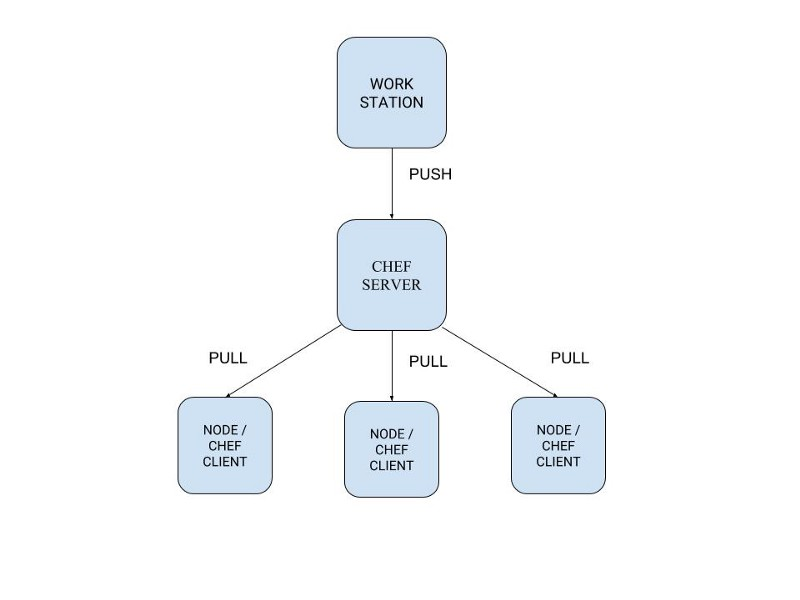
\includegraphics[width=.8\linewidth]{figures/img_Chef_structure.jpeg}
    \caption{Chef Structure}
    \label{fig:chef-structure-image}
\end{figure}

The Infra Server communicates with Infra Clients via HTTP(S) connections.

\subsection{Recipe}
Recipe is the file that contains a set of tasks to be executed step by step in the clients. It has to be in a Cookbook.

\subsection{Resource}
Resource is a piece of code that declares an element of the system and what action should be executed.
Like a sort of module in Ansible, it is possible to set the \textbf{install} and the \textbf{package} to install, for have the desired package installed.

\subsubsection{Services}
Services are used to trigger service status changes, like restarting or stopping a service.

\subsection{Cookbook}
Cookbook is a collection of recipes and other related files organized in a pre-defined way. It is created in a way to simplify the organization and sharing.

\subsection{Attributes}
Attributes are details about a specific node. Can also be defined inside recipes.
It also exists \textbf{automatic attributes} for example contain info about the system.


\subsection{Example of Recipe}
An example of a recipe\cite{chefDigitalOcean}:

\lstinputlisting[label={lst:exampleRecipeChef}]{listings/exampleRecipeChef.rb}

About the recipe:

The recipe starts with an attribute definition, \texttt{node['main']['doc\_root']} where a directory is defined.


At the beginning, there are resources to \texttt{execute} a command (apt-get update), also \texttt{apt\_package} resource to install package apache2.


The service resource enables and starts the service apache2.

\texttt
{directory node['main']['doc\_root'] do [...] end} defines custom attributes for that folder and create it.

A cookbook\_file resource is used to copy a local file to a remote server. This resource will copy \texttt{index.html} file and place it inside the document root created before.


In the end, the template resource applies our Apache virtual host template and notifies the service apache2 for a restart.

\section{Characteristics}

\subsection{Platforms available (Linux, Windows, MacOS)}
At \url{https://docs.chef.io/platforms/} there are written different OSs, with different sections about different Chef modules(like Infra Client, Infra Server, etc.).
The support is described as \textbf{Commercial Support} and \textbf{Community Support}.
The commercial support is described in the official Chef documentation as:
"Commercial support for platforms is part of paid maintenance contracts with Chef Software. Support contracts allow you to open tickets and receive service level agreement (SLA) assistance from our support desk. Commercially supported platforms are extensively tested as part of Chef’s development and release process. Commercial support follows the lifecycle of the underlying operating system vendor.


Commercial support is limited to the platforms listed in the "Commercial Support" tables.
Platforms not listed in those are unsupported"\cite{chefDocPlatforms}.

Instead, the Community Support is considered but differently:
"Community support for platforms means that members of the Chef community have contributed to these platforms and Chef doesn't actively work to maintain this functionality. Chef doesn't explicitly test community-supported platforms as part of the development and release process.

Many of these are forks, clones, or otherwise derivative of platforms that Chef commercially supports.
Continued functionality for these platforms is likely, but not guaranteed.
Unsupported platforms may have missing or non-operative functionality.
As always, we welcome community contributions from anyone
looking to expand community support for platforms in Chef products"\cite{chefDocPlatforms}.


There is also support for \textbf{Derived Platforms}, for example for a distribution that is rebuilt on an original supported distribution.

For Example, \texttt{Chef Infra Client} has Commercial Support for Amazon Linux, CentOS, Debian, FreeBSD, Ubuntu, and other Linux distros but also MacOS and Windows.
It has also derived support for AlmaLinux, whose parent is CentOS but also a lot of Community Support platforms like Arch, Kali, Mint and others.

\subsection{Chef project}
The open source projects published by Chef are under Apache 2.0 license.
The main repo for Chef open source projects is \url{https://github.com/chef/}.
The Chef Server is written almost completely in Erlang and also Ruby.
The Chef Infra Language is a comprehensive systems configuration language, based on Ruby, with resources and helpers for configuring operating systems. The language is primarily used in Chef Infra recipes and custom resources to tell the Chef Infra Client what action(s) to take to configure a system\cite{chefInfraLanguage}.
Ruby is a free and open-source language that is not the simplest but it is used for different uses, its first release was in 1995.

\subsection{Architecture, agent or agentless}
Chef works on client-server configuration with the addition of a workstation.
In Chef, there is an architecture where nodes pull configurations from the server. Chef has its server as the source of truth that requires uploaded cookbooks.
The server runs on the master machine, while the client runs as an agent on every node. Chef also has an extra component named “workstation” that stores all of the configurations that are tested and then pushed to the central server.


A simplified image from the official documentation:

\begin{figure}[H]
    \centering
    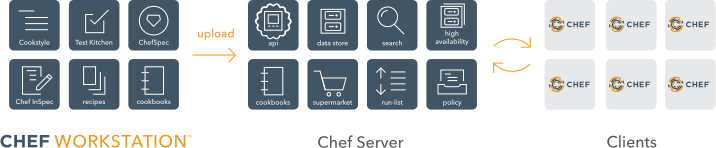
\includegraphics[width=.8\linewidth]{figures/chef_infra.png}
    \caption{Chef Infra}
    \label{fig:chef-infra-image}
\end{figure}

\subsection{Extensions of the project}
It is possible to use Cookbooks (and Chef tools) created by the community, uploaded in the \textbf{Supermarket} and publicly available at \url{https://supermarket.chef.io/}.


"Chef Supermarket is the site for community cookbooks. It provides a searchable cookbook repository and a friendly web UI. Cookbooks that are part of the Chef Supermarket are accessible to any Chef user.


There are two ways to use Chef Supermarket:


The public Chef Supermarket is hosted by Chef Software and is located at Chef Supermarket.


A private Chef Supermarket may be installed on-premise behind the firewall on the internal network. Cookbook retrieval from a private Chef Supermarket is often faster than from the public Chef Supermarket because of closer proximity and fewer cookbooks to resolve. A private Chef Supermarket can also help formalize internal cookbook release management processes (e.g. “a cookbook is not released until it is published on the private Chef Supermarket”)."\cite{chefSupermarket}

\section{Installation}
The Chef Software install script can be used to install any Chef Software, including things like Chef Infra Client, Chef Infra Server, and Chef InSpec.


This script does the following:
\begin{itemize}
    \item Detects the platform, version, and architecture of the machine on which the installer is being executed
    \item Fetches the appropriate package, for the requested product and version
    \item Validates the package content by comparing SHA-256 checksums
    \item Installs the package
\end{itemize}


\cite{chefDocInstall}

\subsection{Example}

For UNIX, Linux, and MacOS systems (insert password when required), via terminal:


\begin{lstlisting}
curl -L https://omnitruck.chef.io/install.sh | sudo bash
\end{lstlisting}


For Windows systems, via PowerShell:
\begin{lstlisting}
. { iwr -useb https://omnitruck.chef.io/install.ps1 } | iex; install
\end{lstlisting}


\cite{chefDocInstall}

\section{Tecnologies for testing Chef}
In Chef, like others, it is possible to simply check the syntax with a single command via the terminal.
For exemple\cite{chefTestMedium}
\begin{lstlisting}
    chef exec ruby -c test-cookbook/recipes/test-recipe.rb
\end{lstlisting}


There is an entire suite for testing called Test Kitchen \url{https://kitchen.ci/} directly supported by Chef.
Test Kitchen provides a test harness to execute infrastructure code on one or more platforms in isolation.\cite{chefTestKit}
Test Kitchen is used by all Chef-managed community cookbooks and is the integration testing tool of choice for cookbooks.\cite{chefTestKit}
There is also an official Chef guide, is explains the power of using Chef Workstation and Test Kitchen together, at \url{https://www.chef.io/docs/cheflibraries/product-and-user-guides/chefguide_test_kitchen.pdf}.
Chef Workstation also includes InSpec, which is an open-source framework for testing and auditing your applications and infrastructure. It compares the actual state of your system with the desired state that you express in easy-to-read and easy-to-write Chef InSpec code. It detects violations and displays findings in the form of a report, but puts you in control of remediation.\cite{chefInSpec}
Test Kitchen allows you to apply your Chef Infra cookbooks and recipes to a variety of machines. It is immediately possible to verify the results with Chef InSpec, ensuring that those systems are properly deployed and remain in the states you want.\cite{chefTestKitPdf}

\section{Learning curve}
Even if it is not the simplest, Chef has a good community with actively supports the technology and other developers.
The Infra Client is written in Ruby but the server is a mix of Erlang and Ruby for most of the part.
The Chef Infra Language, based on Ruby, is not difficult to understand but it is not the simplest language, in fact, in the official documentation of Ruby it is possible to read about Ruby that the creator, Yukihiro Matsumoto, "trying to make Ruby natural, not simple"\cite{rubyDoc}.

%***********************************
%*** PUPPET
%***********************************
\chapter{Puppet}
Puppet is an open source project, with an active community, that invites you to engage with the community to share knowledge and expertise.
Puppet works defining a desired state. Different from other languages, Puppet uses its language Puppet's Domain-Specific Language (DSL), called Puppet code.
It has a high flexibility in the system where it can be used, so it has compatibility with different platforms.
\textbf{Puppet code} is a declarative language, and Puppet works defining the state desired. Puppet then automates putting the system into the state described.
The Puppet Server stores the code that defines your desired state and the Puppet agent translates your code into commands and then executes it on the systems you specify, in what is called a Puppet run.
\cite{puppetDocIndex}
\cite{puppetDocWhatIs}

\section{The beginning of Puppet}

\subsection{History}
Puppet began in 2005 by Luke Kanies
"Luke Kanies is the Founder and CEO of Clickety. He also founded Puppet and Puppet Labs in 2005 out of fear and desperation, with the goal of producing better operations tools and changing how we manage systems.


He has been publishing and speaking on his work in system administration since 1997, focusing on development since 2001. He has developed and published multiple simple sysadmin tools and contributed to established products like Cfengine, and has presented on Puppet and other tools around the world, including at OSCON, LISA, Linux.Conf.au, and FOSS.in. His work with Puppet has been an important part of DevOps and delivering on the promise of cloud computing".\cite{puppetStory1}


In 2010, "Data center automation company Puppet Labs has acquired an open source project called The Marionette Collective. The project, also known as the Mcollective, is a framework to build server orchestration or parallel job execution systems".\cite{puppetStory2}
The open source project acquired aims to programmatically execute actions on clusters of servers.
This acquisition wishes to help provide multi-server and multi-datacenter orchestration for the companies that use Puppet Labs framework for systems management.
The Marionette Collective's real-time capabilities for networking made it simpler to schedule complex sequences of activities using data available from the Puppet platform.\cite{puppetStory2}


In 2011 version 2.0 of Puppet was announced with some interesting features. These include new orchestration capabilities that give systems administrators “command and control”
power to efficiently make parallel changes across clusters of nodes with just a single
command. Also, there were new baselining capabilities that enabled systems administrators to monitor their
infrastructure's compliance against a desired state, a critical input to comprehensive
change management and auditing processes\cite{puppetStory3}.


In 2017, Puppet announced that it had acquired Distelli, a Seattle startup founded in 2015 by Singh that helps software engineers deploy code more efficiently.\cite{puppetStory4}
About that acquisition, Puppet Chief Product Officer that was at that time Omri Gazitt who said “We quickly realized Distelli represented the best of everything that we were hoping to get” and “matched perfectly with our philosophy”\cite{puppetStory4}.


In 2022, Perforce acquired Puppet, as described on the official Perforce site:
"Perforce Software (“Perforce”), a provider of solutions to enterprise teams requiring productivity, visibility, and scale along the development lifecycle, backed by Francisco Partners and Clearlake Capital Group, L.P. (together with its affiliates, “Clearlake”), announced today that it has signed a definitive agreement to acquire Puppet (or “the Company”), an infrastructure automation software platform which enables users to deliver, update, monitor, and secure software across physical and virtual machines"\cite{puppetStory5}.


Over the years, Puppet has grown raising money and growing its set of technological partners.
Now it has its 8.4.x version.

\section{Purpose of the technology}
Puppet is a project proud to be open source, it encourages a lot of the participation of the community.
It creates a sort of group to thank with some benefits dedicated to that, called "Puppet Champion", and also a special group called "The League of Extraordinary Puppeteers"\cite{puppetDocChampions}.


Puppet is built on the concept of IaS (Infrastructure as Code), meaning that the infrastructure is created by writing code by the system administrator adopting practices that are traditionally associated with software developers.
It enables system administrators to define infrastructure using code written in the Puppet Descriptive Language, eliminating the need for custom scripts.


Idempotency is considered a key feature of Puppet, allowing Puppet to run continuously, obtaining the same system state result every time.
It ensures that the state of the infrastructure always matches the desired state.
If there are any changes not made on purpose to the system's state described, Puppet can rectify those changes and restore the system to its desired state.


Puppet offers a scalable solution, that allows the system administrators to centralize and streamline automations across multiple machines.


When adopting a tool like Puppet, Puppet itself advises using it with an agile methodology in mind (making incremental units of work and reusing code).
With more familiarity with Puppet, more scalability is possible. And also agile invites colleagues to spread the work between them.
Sharing common Puppet methodology and language between colleagues allows the business to work more efficiently.
\cite{puppetIntroMedium}\cite{puppetDocIntro}


There are some Puppet use cases, for example, Alex Zbarcea, DevOps Engineer III, Fannie Mae said "Puppet forces you to have accountability for each artifact managed in production. You'll know nothing is being missed, nothing is not being tracked. Puppet brings a lot of health into configuration management, giving visibility to teams across silos so they know the lifecycle of each artifact for services required for other services. Puppet is great at answering: Are the services configured as they should be? Did anything change? Is there a conflict between configuration processes? Puppet brings consistency and predictability into the environment. When you have to upgrade a service, it's so much easier"\cite{puppetDocUseCase}.


\subsection{Best points of Puppet}

Some Puppet key features:

\begin{itemize}
    \item \textbf{Idempotency}: Execute automations code once, is equal to executing hundreds of times. When the state is defined, the system forces to obtain(or maintain) the state desired of the system.
    \item \textbf{Promote community}: Puppet gives some benefits (like discount, contents, stickers) to the contributors that are in a "group" called Puppet Champion".
    There is also a special group called "The League of Extraordinary Puppeteers" that can you enter on it only by community nomination (and offers additional benefits).
    \item \textbf{DevOps oriented}: Puppet wishes to work in a agile style inviting system administration to use devops technologies and practice
    \item \textbf{Mature industry-proven technology} It has a strong user base, used by from community users to big tech companies (Accenture, Uber, Twich), it has been created years before different competitors and has great documentation on itself sources and also on others related online resources.
\end{itemize}

\section{How the tool is shown to the community}

\subsection{Who supports and maintains the project}
The project is supported by the community and also by the company that acquired it some years ago \textbf{Perforce}.

\subsection{Statistics}

Puppet has 
\begin{itemize}
    \item 7.2k stars
    \item $>$450 watcher
    \item 2.2k fork
    \item 19 issue with 7 closed
    \item $>$30 pull request
    \item $>$580 contributors
    \item 12.2k projects use it as a dependency
\end{itemize}
\cite{puppetGitHubProject}
We could consider the community active as contributors and very used as a dependency. There are not a lot of issues and pull requests. Anyway, it has a lot of stars and forks.

\subsection{Community way to help and improve}
The main GitHub community page has a photo and also a description of the Puppet community:
"At Puppet, open source software is in our DNA. From the earliest days of Facter to the latest version of Bolt, we've always been firm believers in the power of open source. We have a supportive, active community of thousands of people just like you who are making Puppet better — and making IT a better place to work"\cite{puppetGitHubGeneral}.

There are also many channels available to contribute/participate in the community:
\begin{itemize}
    \item Slack at \url{https://slack.puppet.com}
    \item Tickets at \url{https://tickets.puppet.com}
    \item Forge at \url{https://forge.puppet.com}
    \item Voxpupuli at \url{https://voxpupuli.org} (described as "collective of Puppet module, tooling and documentation authors all working together to ensure continued development on the code we maintain")\cite{puppetVox}
    \item dev.to and dev.to feed at \url{https://dev.to/puppet}, \url{https://dev.to/feed/tag/puppet}
    \item Mastodon at \url{https://fosstodon.org/@puppet}
    \item GitHub discussion at \url{https://github.com/puppetlabs/community/discussions}
\end{itemize}

There are some different opportunities described at \url{https://www.puppet.com/community}.
For example, three Mailing List on Google Groups at \url{https://groups.google.com/g/puppet-users?pli=1}, \url{https://groups.google.com/g/puppet-announce}, \url{https://groups.google.com/g/puppet-security-announce}.


There is a calendar with meetings, streams, etc. at \url{https://www.puppet.com/community/calendar}.
There is a dedicated customer experience research program for the community, called Puppet Test Pilots. It offers benefits like gift cards or charity donations for participating, at \url{https://www.puppet.com/community/puppet-test-pilots}.
There is a Puppet Dev Kit at \url{https://www.puppet.com/community/open-source} to develop and test Puppet modules by providing a simple, unified interface to a set of helpful tools for anyone who writes or consumes Puppet code\cite{puppetDocDevKit}.

Other particular programs are Puppet Champions and The League of Extraordinary Puppeteers.
Puppet Champions is a group that allows you to have some benefits like Puppet presentations, demos, Puppet store discounts, stickers, etc.
The Extraordinary Puppeteer is a distinction that is available only by peer nomination for the most passionate Champions. It includes additional benefits like advisory board participation, travel scholarships, etc.


Some of those ideas are not present in other automation tools, and that means that Puppet is not only open but also willing to take contributions.

\section{Main Puppet components}

There are main components of Puppet, with also some graphics related.

\textbf{Facter}

In Puppet there is an inventory tool called Facter. The agent sends these facts to the primary server.
It is possible to add custom facts by writing snippets of Ruby code on the primary Puppet server. Puppet then uses plug-ins in modules to distribute the facts to the client.
It exists \texttt{external facts} that provide a way to use arbitrary executables or scripts as facts, or set facts statically with structured data.
It has also a configuration file called \textbf{facter.conf} that allows the user to cache and block fact groups and facts, and manage how Facter interacts with the system.

\cite{puppetDocPlatform} \cite{puppetDocFacter}

\textbf{Catalog}
Catalog is a JSON document that describes the desired state of a specific agent node, created with facts received from Facter.
Each agent requests and receives its own individual catalog and then enforces that desired state on the node it's running on.
Puppet is so able to apply changes all across the entire infrastructure, ensuring that each node matches the state is defined with Puppet code. \cite{puppetDocPlatform}

\textbf{Modules}
Modules serve as the basic building blocks of Puppet and are reusable and shareable.
You keep nearly all of your Puppet code in modules that contain both code and data.
Using a tool called Hiera, you can separate the data from the code and place it in a centralized location.
Each module manages a specific task in the infrastructure, such as installing and configuring a piece of software.
Modules contain Puppet classes, defined types, tasks, task plans, functions, resource types and providers, and plug-ins such as custom types or facts. 
\cite{puppetDocPlatform} \cite{puppetDocModules}

\textbf{PuppetDB}
All of the data generated by Puppet (for example facts, catalogs, reports) is stored in the Puppet database (PuppetDB).
Storing data in PuppetDB allows Puppet to work faster and provides an API for other applications to access Puppet's collected data.
Once PuppetDB is full of your data, it becomes a great tool for infrastructure discovery, compliance reporting, vulnerability assessment, and more. These task can be done via PuppetDB queries. \cite{puppetDocPuppetDB}

\textbf{Puppet agent}
Puppet agent is the application that manages configurations on your nodes. It requires a Puppet primary server to fetch configuration catalogs.
Puppet agent runs as a specific user, (usually root) and initiates outbound connections on port 8140.

Each node executes periodic configuration runs, to avoid unattended changes and make updates.

That can be done with:
\begin{itemize}
    \item Run Puppet agent as a service
    The Puppet agent daemon does configuration runs at a set interval, which can be configured.
    \item Make a cron job that runs Puppet agent (not for Windows)
    Reduce the number of persistent processes on the systems, but require more manual configuration.
    \item Only run Puppet agent on demand.
    To run on demand on many nodes it is possible to use Bolt \url{https://www.puppet.com/docs/bolt/} or deploy MCollective \url{https://forge.puppet.com/modules/puppet/mcollective/readme}.
\end{itemize}

\cite{puppetDocAgentNix} \cite{puppetDocAgentWin}

\textbf{Puppet device}
With Puppet device, you can manage network devices, such as routers, switches, firewalls, and IoT devices, without installing a Puppet agent on them. \cite{puppetDocDevice}

\textbf{Puppet apply}
Puppet apply is an application that compiles and manages configurations on nodes. It acts like a self-contained combination of the Puppet primary server and Puppet agent applications. \cite{puppetDocApply}

\textbf{Puppet reports}
Puppet creates a report about its actions and your infrastructure each time it applies a catalog during a Puppet run. You can create and use report processors to generate insightful information or alerts from those reports. \cite{puppetDocReports}

\begin{figure}[H]
    \centering
    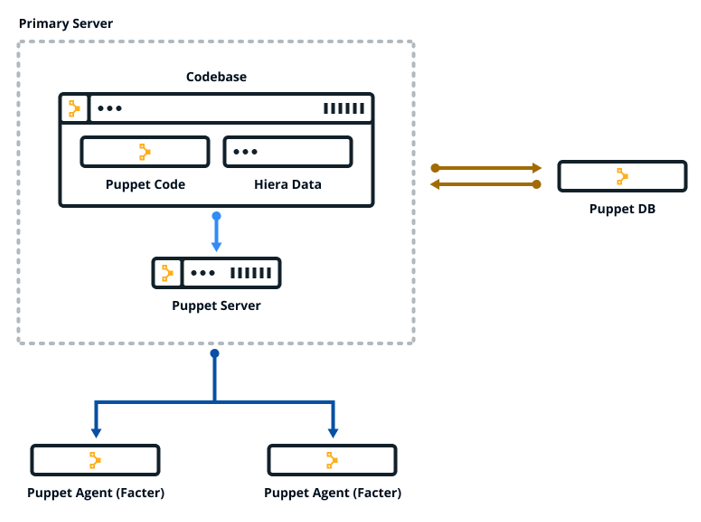
\includegraphics[width=.8\linewidth]{figures/puppetplatformjpeg.png}
    \caption{Puppet Platform}
    \label{fig:puppet-platform-image}
\end{figure}\cite{puppetDocPlatform}

\begin{figure}[H]
    \centering
    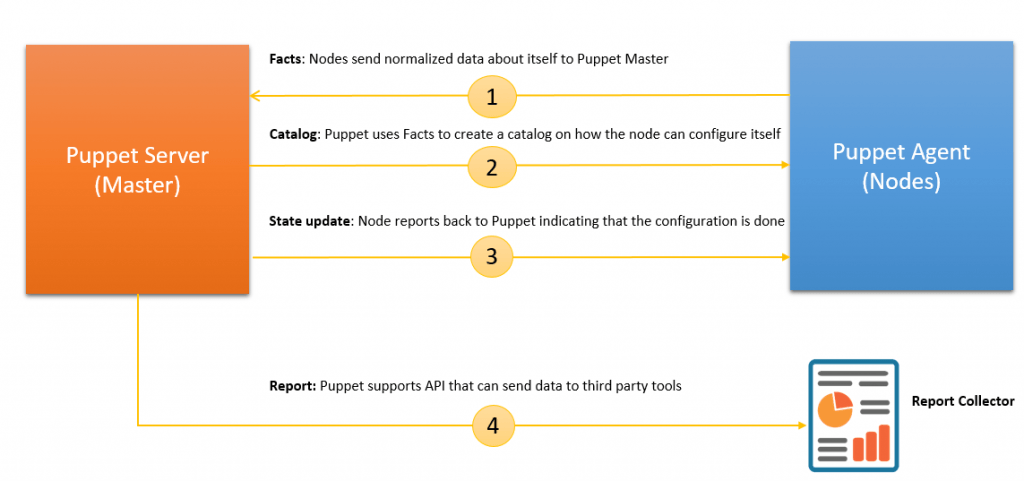
\includegraphics[width=.8\linewidth]{figures/puppetfunctioning.png}
    \caption{Puppet Functioning}
    \label{fig:puppet-functioning-image}
\end{figure}\cite{puppetImgFunctioning}

\subsection{Platforms available (Linux, Windows, MacOS)}

About Puppet Server, Puppet provides official packages that install Puppet Server and all of its prerequisites for the following platforms:

\begin{itemize}
    \item Red Hat Enterprise Linux vers. 7,8,9
    \item Debian vers. 9,10,11
    \item Utuntu vers. 16.04 (amd64 only), 18.04, 20.04, 22.04
    \item SUSE Enterprise Linux vers. 12 SP1, 15 (x86\_64)
\end{itemize}

If Puppet doesn't provide a package for your system, you can run Puppet Server from source on any x86\_64 Linux server with JDK 1.8 or 11.
\cite{puppetDocSupportServer}

About Puppet agent, the installation is instead available for *nix, Windows, or MacOS.
\cite{puppetDocSupportAgents}

\subsection{Puppet project}
The general Puppet project is available at \url{https://github.com/puppetlabs/}.
The part related to the Puppet main project at \url{https://github.com/puppetlabs/puppet}.

This project is written in Ruby, available with Apache License 2.0\cite{puppetGitHubProject}.
About the choice to write Puppet in Ruby instead in a language as Python, Luke Kanies, the author of Puppet said "I tried Python, because this was around 2003 and Python was the next new thing and everyone was saying how great it is, but I just can't seem to write in Python at all. A friend had said he'd heard Ruby was cool, so I gave it a try, and in four hours I went from never having seen a line of it to having a working prototype. I haven't looked back since then, and haven't regretted the choice"\cite{puppetDocOldFAQ}.

Puppet automations is defined in a declarative language derived from Ruby (Ruby DSL) called Puppet Code.

\subsection{Architecture, agent or agentless}
Considering that Puppet automation is described in Puppet Code that is declarative, the automations work describing the state the desired state of the system and not the steps needed to get there.
Puppet then automates the process of getting these systems into that state and keeping them there.
Puppet does this through Puppet primary server and a Puppet agent.
The Puppet primary server is the server that stores the code that defines your desired state.
The Puppet agent translates your code into commands and then executes it on the systems you specify, in what is called a Puppet run\cite{puppetDocWhatIs}.
In Puppet servers and agents communicate by HTTPS using SSL certificates. Puppet includes a built-in certificate authority for managing certificates.Puppet Server performs the role of the primary node and also runs an agent to configure itself\cite{puppetDocPlatform}.

\begin{figure}[H]
    \centering
    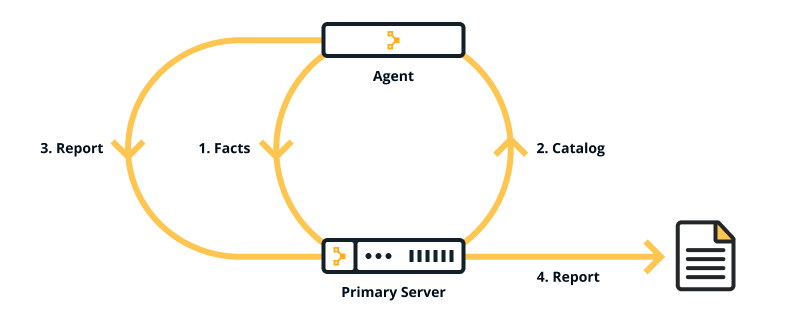
\includegraphics[width=.8\linewidth]{figures/puppetagentserverjpeg.png}
    \caption{Puppet Agent Server}
    \label{fig:chef-agent-server-image}
\end{figure}\cite{puppetDocWhatIs}

\subsection{Extensions of the project}
It is possible to create custom code and modules, using the \textbf{Puppet Development Kit (PDK)}.
PDK is "a framework to successfully build, test and validate your modules"\cite{puppetDocPDK}.


There is also a sort of collection of modules called \textbf{Puppet Forge} at \url{https://forge.puppet.com/}.
"Puppet Forge is a catalogue of modules created by Puppet, our partners, and community that helps IT ops practitioners supercharge and simplify their automation processes. With step-by-step guides and tutorials, Puppet Forge provides a platform for you to grow your skills with Puppet, whatever your current level"\cite{puppetForge}.
Puppet Forge modules could have different badges like "Supported" or "Approved" by Puppet.
There are more than 7k modules available and about 2.5k community contributors.

Considering the Puppet community and related channels, there is a project called Vox Populi, which defines itself as "We are a collective of Puppet module, tooling and documentation authors all working together to ensure continued development on the code we maintain"\cite{puppetVox}.
About the way works this project "We work under a shared name and namespace and synchronize our efforts. Having no official relation to Puppet Inc. allows us to maintain our own pace and direction when it comes to how we work and develop"\cite{puppetVox}.

\section{Installation}

\subsection{Enable the Puppet platform repository}
First of all, to install Puppet on the system is necessary to enable the Puppet platform repository.
Enabling the Puppet platform repository makes the components needed for installation available on your system.
The enabling of the repository depends on which package management system the system uses: \texttt{yum} or \texttt{apt}.
It is important to search the correct URL of the package to enable based on the operating system and version, located in \url{yum.puppet.com} and \url{apt.puppet.com}.
\cite{puppetDocInstall}

\subsubsection{Example for Yum}
Logged in as root, run the RPM tool in upgrade mode.
\begin{lstlisting}
sudo rpm -U <PACKAGE_URL>
\end{lstlisting}

Example to enable the Enterprise Linux 8 repository. 
\begin{lstlisting}
sudo rpm -Uvh https://yum.puppet.com/puppet8-release-el-8.noarch.rpm
\end{lstlisting}

\subsubsection{Example for apt}
Logged in as root, download the package and run the dpkg tool in install mode.
\begin{lstlisting}
wget <PACKAGE_URL>
sudo dpkg -i <FILE_NAME>.deb
\end{lstlisting}

Example to enable the Ubuntu 20.04 focal repository.
\begin{lstlisting}
wget https://apt.puppet.com/puppet8-release-focal.deb
sudo dpkg -i puppet7-release-focal.deb
\end{lstlisting}

Update the apt package lists.
\begin{lstlisting}
sudo apt-get update
\end{lstlisting}

\cite{puppetDocInstall}

\subsection{Install Puppet Server}
Install the Puppet Server package.


On Red Hat OS:
\begin{lstlisting}
yum install puppetserver
\end{lstlisting}

On Debian and Ubuntu OS:
\begin{lstlisting}
apt-get install puppetserver
\end{lstlisting}

Start the Puppet Server service.
\begin{lstlisting}
sudo systemctl start puppetserver
\end{lstlisting}

Open a new shell, or use \texttt{exec bash} to update your PATH (or \texttt{bash -l} on Ubuntu).


Check if Puppet Server is installed correctly.
\begin{lstlisting}
puppetserver -v
\end{lstlisting}


Puppet Server is configured to use 2GB of RAM. However, it is possible to test it also on a VM, allocating as little as 512MB of memory. 

\cite{puppetDocSupportServer}

\subsection{Install Puppet agents}
There are different ways to install Puppent agents, also considering that it is possible to install them not only in Linux but also in Windows and MacOS.
In Linux, after enabling Puppet platform repository, install the agent by the terminal using the command appropriate to the OS environment and start the Puppet service.
In Windows, it is possible to use msi package to install agent. It is also possible to upgrade or downgrade between 32-bit and 64-bit Puppet on Windows nodes.
In MacOS, there are different ways to install agent: from Finder, the command line or Homebrew.

\cite{puppetDocSupportAgents}

\section{Tecnologies for testing Puppet}
One way to test modules is using \textbf{Litmus}, which is installed as (experimental) part of Puppet Development Kit(PDK). It is "a command line tool that allows you to run acceptance tests against Puppet modules for a variety of OSes and deployment scenarios"\cite{puppetLitmus}.

PDK includes a series of tools to test Puppet, not only for modules but also for code, such as:
\begin{itemize}
    \item \textbf{puppet-lint} checks that Puppet manifests conform to the style guide\newline
    https://github.com/puppetlabs/puppet-lint
    \item \textbf{metadata-json-lint} validates and lint Puppet metadata.json files\newline
    https://github.com/voxpupuli/metadata-json-lint
    \item \textbf{puppetlabs-rspec} tests for Puppet manifests and modules\newline
    https://github.com/puppetlabs/rspec-puppet
    \item \textbf{rspec-puppet-facts} simplify unit tests by looping on every supported Operating System and populating facts\newline
    https://github.com/voxpupuli/rspec-puppet-facts
\end{itemize}
Some of them are from \texttt{Vox Populi}, where there are many tools created by the community to execute different tests.
There are some test tools created by the community also on \texttt{Puppet Forge}.
It also exists a Puppet Extension for Visual Studio Code and a Puppet Plugin for IntelliJ Idea.

\section{Learning curve}
It is possible to consider Puppet learning curve not one of the fastest.
Puppet project is written in Ruby, which is not as simple as language for beginners like Python.
Puppet automations are not written in Ruby but in a Ruby DSL which adds another little difficulty to start with Puppet.
About the fact that Puppet wish not to use XML/YAML for automations, it is beacuse "using XML or YAML would limit any assurance that the interface was declarative - one process might treat an XML configuration differently from another"\cite{puppetDocOldFAQ}.
Considering also that the Puppet structure is not a standard agent-server structure it is not the best for beginners in automations, but has good support from the community.

\chapter{Conclusion}

\subsection{Comparison}
%Make table with comparison about
%differences and similarity
%(modification are possible)
%structure
%learning curve
%languages used
%community

\subsection{Consideration}
%Consideration about the thesis and what I learned


%----------------------------------------------------------------------------------------
% BIBLIOGRAPHY
%----------------------------------------------------------------------------------------

\backmatter

\nocite{*} % comment this to only show the referenced entries from the .bib file

\bibliographystyle{plainnat}
\bibliography{bibliography}

\end{document}